\documentclass[aspectratio=169,11pt]{beamer}

\usetheme{Madrid}
\usecolortheme{default}

\usepackage[T1]{fontenc}
\usepackage[utf8]{inputenc}
\usepackage{booktabs}
\usepackage{graphicx}
\usepackage{amsmath}
\usepackage{array}
\usepackage{hyperref}
\usepackage{tikz}
\usetikzlibrary{arrows.meta}

\hypersetup{
  colorlinks=true,
  urlcolor=blue,
  linkcolor=blue
}

\setbeamertemplate{navigation symbols}{}
\setbeamertemplate{footline}[frame number]
\setbeamerfont{title}{size=\Large}
\setbeamerfont{frametitle}{size=\large}

\title[Faithfulness Under Pressure]{Faithfulness Under Pressure}
\subtitle{Context and History Pruning for Conversational RAG Faithfulness}
\author[M. G\"uden, B. F. Tekin]{Mert G\"uden \and Berkay Fehmi Tekin}
\institute[CENG 467]{CENG 467 -- Natural Language Understanding and Generation}
\date{June 2026}

\begin{document}

\begin{frame}
  \titlepage
\end{frame}

\begin{frame}{Problem}
  \begin{block}{Question}
    When a small language model receives long, noisy retrieved context, can pruning make its answer more faithful to the evidence?
  \end{block}

  \vspace{0.5em}
  \begin{itemize}
    \item Task: conversational open-domain question answering with RAG.
    \item Main benchmark: QReCC, where each question depends on previous conversation turns.
    \item Output: short answer generated from retrieved/pruned evidence and retained dialogue history.
    \item Main risk: the model may keep stale history, miss the current evidence, or hallucinate unsupported claims.
  \end{itemize}
\end{frame}

\begin{frame}{Why Pruning Matters}
  \begin{columns}[T,onlytextwidth]
    \column{0.52\textwidth}
    \textbf{Long context is not free.}
    \begin{itemize}
      \item More tokens increase latency and memory cost.
      \item Retrieved passages and old dialogue turns often contain near-misses, stale entities, and distractors.
      \item Small LMs are especially sensitive to noisy evidence.
    \end{itemize}

    \column{0.44\textwidth}
    \textbf{Long context is not always used well.}
    \begin{itemize}
      \item Liu et al. show that models often perform best when relevant information is near the beginning or end of the context.
      \item Performance can drop when evidence is in the middle, even for long-context models.
    \end{itemize}
  \end{columns}

  \vspace{0.5em}
  \footnotesize Source: Liu et al., TACL 2024, ``Lost in the Middle''.\footnote{\url{https://aclanthology.org/2024.tacl-1.9/}}
\end{frame}

\begin{frame}{Project Pipeline}
  \centering
  \small
  \begin{tabular}{c}
    \fbox{QReCC conversational turn + history} \\
    $\downarrow$ \\
    \fbox{Optional rewrite / current-turn query} \\
    $\downarrow$ \\
    \fbox{Retriever: top-k passages} \\
    $\downarrow$ \\
    \fbox{Context + history pruner} \\
    $\downarrow$ \\
    \fbox{Mistral-7B-Instruct Generator} \\
    $\downarrow$ \\
    \fbox{LLM-as-Judge Faithfulness Scoring}
  \end{tabular}

  \vspace{0.35em}
  \begin{itemize}
    \item The retriever and generator are held fixed across pruning strategies.
    \item Only retrieved context and retained history change.
    \item This isolates the effect of pruning on faithfulness, answer quality, and compression.
  \end{itemize}
\end{frame}

\begin{frame}{Pruning Strategies}
  \small
  \begin{tabular}{p{0.16\textwidth}p{0.28\textwidth}p{0.44\textwidth}}
    \toprule
    ID & Strategy & Role \\
    \midrule
    B1 & No pruning & Full retrieved context; maximum evidence and maximum noise. \\
    B2 & Naive truncation & Hard token budget; common but relevance-agnostic. \\
    B3 & RECOMP-style extractive & Selects query-relevant sentences from retrieved passages. \\
    S1 & LLMLingua-2 & Token-level compression using a bidirectional encoder classifier. \\
    S2 & Provence & Sentence-level sequence-labeling pruner, also related to reranking. \\
    S3 & History pruning & Removes redundant context using conversation history. \\
    S4 & Combined & Sentence pruning plus history-aware pruning. \\
    S5 & CfC/LNN extension & Exploratory adaptive pruning model for multi-turn context. \\
    \bottomrule
  \end{tabular}
\end{frame}

\begin{frame}{Related Work Signals}
  \begin{itemize}
    \item \textbf{RECOMP}: compresses retrieved documents before generation; reports compression rates as low as 6\% with minimal performance loss in evaluated settings.\footnote{\url{https://proceedings.iclr.cc/paper_files/paper/2024/hash/bda88ed2892f5e61c9a9bf215c566913-Abstract-Conference.html}}
    \item \textbf{LLMLingua-2}: formulates prompt compression as token classification and reports 1.6--2.9$\times$ end-to-end latency acceleration at 2--5$\times$ compression.\footnote{\url{https://huggingface.co/papers/2403.12968}}
    \item \textbf{Provence}: treats context pruning as sequence labeling and reports negligible to no performance drop at almost no additional RAG pipeline cost.\footnote{\url{https://arxiv.org/abs/2501.16214}}
  \end{itemize}

  \vspace{0.5em}
  \begin{block}{Our angle}
    We use QReCC because the central problem is conversational: deciding which past turns and retrieved passages still matter for the current question.
  \end{block}
\end{frame}

\begin{frame}{Dataset and Experimental Setup}
  \begin{columns}[T,onlytextwidth]
    \column{0.48\textwidth}
    \textbf{Main benchmark: QReCC}
    \begin{itemize}
      \item 14K conversations.
      \item About 81K question-answer pairs.
      \item Built for question rewriting in conversational context.
      \item Retrieval collection: 10M web pages split into 54M passages.
      \item Each sample includes original question, context, rewrite, answer, and answer provenance.
    \end{itemize}

    \column{0.48\textwidth}
    \textbf{Current experiment status}
    \begin{itemize}
      \item Faithfulness: fraction of generated claims supported by context.
      \item EM/F1: lexical answer correctness against gold answer.
      \item Compression ratio: output tokens / input tokens.
      \item History retention: retained turns / original turns.
      \item Pilot HotpotQA runs remain only as implementation sanity checks.
    \end{itemize}
  \end{columns}

  \vspace{0.5em}
  \footnotesize Source: Anantha et al., NAACL 2021 / QReCC dataset release.\footnote{\url{https://aclanthology.org/2021.naacl-main.44/}}
\end{frame}

\begin{frame}{Pilot Results: HotpotQA Sanity Run}
  \small
  \begin{tabular}{lccccc}
    \toprule
    Strategy & Faith. & EM & F1 & Comp. & Lat. s \\
    \midrule
    B1: No pruning & 0.718 & 0.040 & 0.148 & 1.000 & 6.76 \\
    B2: Naive truncation & 0.621 & 0.040 & 0.139 & 0.918 & 4.95 \\
    B3: RECOMP & \textbf{0.750} & 0.040 & 0.141 & 0.911 & 5.38 \\
    S1: LLMLingua-2 fallback & \textbf{0.750} & 0.040 & 0.141 & 0.911 & 5.38 \\
    S2: Provence & 0.657 & 0.000 & 0.057 & \textbf{0.072} & \textbf{4.49} \\
    S3: History, empty & 0.718 & 0.040 & 0.148 & 1.000 & 6.34 \\
    S4: Combined, empty & 0.657 & 0.000 & 0.057 & \textbf{0.072} & \textbf{4.48} \\
    \bottomrule
  \end{tabular}

  \vspace{0.8em}
  \footnotesize Notebook 2, 50 HotpotQA validation samples. These are pilot implementation checks, not the final QReCC benchmark results.
\end{frame}

\begin{frame}{Pilot Results: Gap-Closing Run}
  \small
  \begin{tabular}{lcccccc}
    \toprule
    Strategy & Faith. & EM & F1 & Comp. & Cov. & Noise \\
    \midrule
    B3: RECOMP & 0.648 & 0.080 & 0.195 & 0.962 & \textbf{0.760} & 0.624 \\
    S1: LLMLingua-2 real & \textbf{0.711} & 0.040 & 0.167 & 0.457 & 0.000 & 0.792 \\
    S3: History two-turn & 0.533 & \textbf{0.100} & \textbf{0.214} & 0.962 & 0.627 & 0.641 \\
    S4: Combined two-turn & 0.530 & 0.040 & 0.112 & \textbf{0.081} & 0.222 & \textbf{0.284} \\
    \bottomrule
  \end{tabular}

  \vspace{0.8em}
  \begin{itemize}
    \item LLMLingua-2 is the strongest faithfulness result in this pilot run.
    \item Combined pruning is extremely compact and low-noise, but loses too much support.
    \item QReCC is the correct next benchmark for testing real history pruning.
  \end{itemize}
\end{frame}

\begin{frame}{Faithfulness--Compression Trade-off}
  \centering
  \small
  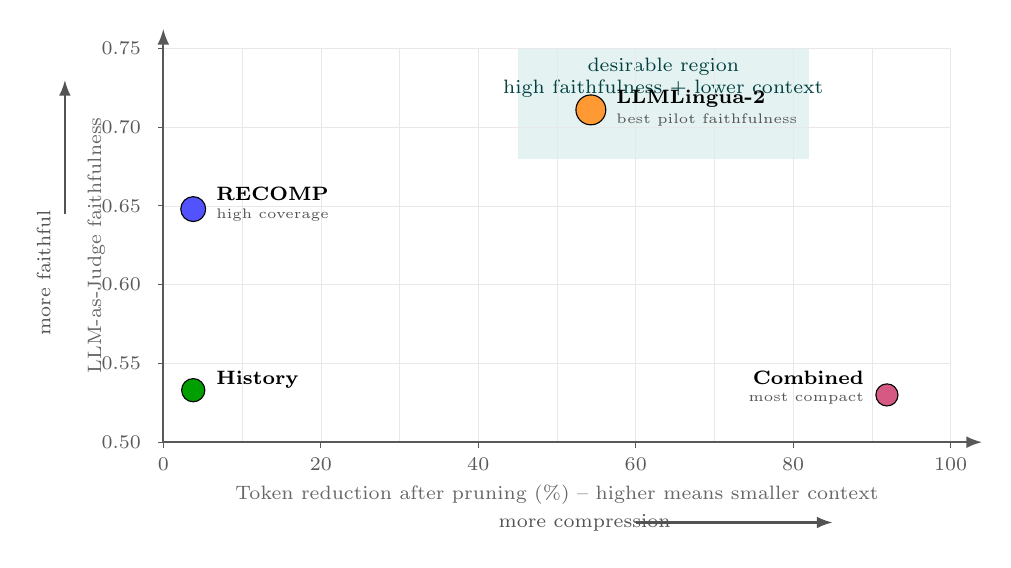
\begin{tikzpicture}[x=1cm,y=1cm]
    % Plot area: x is token reduction 0--100 mapped to 0--10cm.
    % y is faithfulness 0.50--0.75 mapped to 0--5cm.
    \fill[teal!10] (4.5,3.6) rectangle (8.2,5.0);
    \node[align=center, text=teal!50!black, font=\scriptsize] at (6.35,4.63)
      {desirable region\\high faithfulness + lower context};

    \draw[step=1.0, gray!18, very thin] (0,0) grid (10,5);
    \draw[-{Latex[length=2mm]}, thick, gray!70!black] (0,0) -- (10.4,0);
    \draw[-{Latex[length=2mm]}, thick, gray!70!black] (0,0) -- (0,5.25);

    \foreach \x/\label in {0/0,2/20,4/40,6/60,8/80,10/100} {
      \draw[gray!70!black] (\x,0) -- (\x,-0.07);
      \node[font=\scriptsize, text=gray!70!black] at (\x,-0.28) {\label};
    }
    \foreach \y/\label in {0/0.50,1/0.55,2/0.60,3/0.65,4/0.70,5/0.75} {
      \draw[gray!70!black] (0,\y) -- (-0.07,\y);
      \node[font=\scriptsize, text=gray!70!black, anchor=east] at (-0.16,\y) {\label};
    }

    \node[font=\scriptsize, text=gray!80!black] at (5,-0.67)
      {Token reduction after pruning (\%) -- higher means smaller context};
    \node[font=\scriptsize, text=gray!80!black, rotate=90] at (-0.85,2.5)
      {LLM-as-Judge faithfulness};

    % Points. Coordinates are current HotpotQA pilot means:
    % x = (1 - compression_ratio) * 100 / 10, y = (faithfulness - 0.50) * 20.
    \filldraw[fill=blue!68, draw=black, line width=0.4pt] (0.38,2.96) circle (4.5pt);
    \node[anchor=west, font=\scriptsize\bfseries] at (0.55,3.15) {RECOMP};
    \node[anchor=west, font=\tiny, text=gray!65!black] at (0.55,2.88) {high coverage};

    \filldraw[fill=orange!80, draw=black, line width=0.4pt] (5.43,4.22) circle (5.4pt);
    \node[anchor=west, font=\scriptsize\bfseries] at (5.63,4.36) {LLMLingua-2};
    \node[anchor=west, font=\tiny, text=gray!65!black] at (5.63,4.09) {best pilot faithfulness};

    \filldraw[fill=green!62!black, draw=black, line width=0.4pt] (0.38,0.66) circle (4.2pt);
    \node[anchor=west, font=\scriptsize\bfseries] at (0.55,0.80) {History};

    \filldraw[fill=purple!65, draw=black, line width=0.4pt] (9.19,0.60) circle (4.0pt);
    \node[anchor=east, font=\scriptsize\bfseries] at (9.02,0.82) {Combined};
    \node[anchor=east, font=\tiny, text=gray!65!black] at (9.02,0.55) {most compact};

    \draw[-{Latex[length=2mm]}, thick, gray!65!black] (6.0,-1.02) -- (8.5,-1.02);
    \node[font=\scriptsize, text=gray!65!black] at (5.35,-1.02) {more compression};
    \draw[-{Latex[length=2mm]}, thick, gray!65!black] (-1.25,2.9) -- (-1.25,4.6);
    \node[font=\scriptsize, text=gray!65!black, rotate=90] at (-1.52,2.15) {more faithful};
  \end{tikzpicture}

  \vspace{0.15em}
  \scriptsize Current numbers are HotpotQA pilot outputs; final benchmark target is QReCC conversational QA.
\end{frame}

\begin{frame}{What We Learned}
  \begin{itemize}
    \item \textbf{Pruning can improve faithfulness}, but not every pruning method helps equally.
    \item \textbf{Aggressive compression is dangerous for conversational QA}: if the relevant history turn disappears, the current question becomes ambiguous.
    \item \textbf{Faithfulness and correctness are different}: a faithful answer can still be the wrong answer, and a correct short answer can be judged poorly.
    \item \textbf{Exact coverage is too strict for token compression}: LLMLingua-2 may fragment evidence so gold sentences no longer match verbatim.
    \item \textbf{Conversation history is not just extra text}: old turns can help or distract depending on the current question.
  \end{itemize}
\end{frame}

\begin{frame}{Error Analysis Examples}
  \small
  \begin{tabular}{p{0.26\textwidth}p{0.64\textwidth}}
    \toprule
    Error type & Example pattern \\
    \midrule
    Evidence removed & The ``Arizona'' question loses the sentence saying the song was written by Kenny Young. \\
    Verbose correct answer & For yes/no questions, the model may answer correctly with explanation but get EM = 0. \\
    Judge false negative & A short correct phrase such as ``Political correctness'' can be scored as unfaithful. \\
    Entity near-miss & The generator outputs ``T. M. Howard'' instead of ``T. R. M. Howard''. \\
    \bottomrule
  \end{tabular}

  \vspace{0.8em}
  \begin{block}{Takeaway}
    We need judge calibration and qualitative analysis before treating one metric as ground truth.
  \end{block}
\end{frame}

\begin{frame}{CfC / LNN Extension}
  \begin{block}{Motivation}
    Fixed thresholds do not know whether a turn is easy, noisy, redundant, or dependent on earlier dialogue. We want a pruner that adapts over time.
  \end{block}

  \begin{itemize}
    \item We explore continuous-time neural models, especially Closed-form Continuous-time networks (CfCs).
    \item CfCs model temporal dynamics without a heavy numerical ODE solver.\footnote{\url{https://www.nature.com/articles/s42256-022-00556-7}}
    \item In our setting, each utterance or sentence receives an importance score.
    \item The hidden state carries information across conversation turns.
  \end{itemize}
\end{frame}

\begin{frame}{Entropy-Driven CfC Pruning}
  \small
  \textbf{Idea: surprising utterances deserve more processing time.}

  \vspace{0.5em}
  For utterance $u_i$, compute surprisal using a proxy LM:
  \[
    S(u_i) = -\frac{1}{N}\sum_{j=1}^{N}\log P(w_j \mid w_{<j})
  \]

  Map surprisal to a continuous time step:
  \[
    \Delta t_i = \Delta t_{\min} + \beta S(u_i)
  \]

  \begin{itemize}
    \item Input: SBERT embedding of each utterance/sentence plus time step.
    \item Output: importance probability $p_i \in [0,1]$.
    \item Teacher labels: leave-one-out impact on Mistral-7B output.
    \item Training loss: mean squared error between predicted and teacher importance.
  \end{itemize}
\end{frame}

\begin{frame}{CfC Evaluation Plan}
  \begin{columns}[T,onlytextwidth]
    \column{0.48\textwidth}
    \textbf{Baselines}
    \begin{itemize}
      \item Full context.
      \item Random pruning.
      \item Cosine-similarity history pruning.
      \item Existing sentence/token LNN pruners.
    \end{itemize}

    \column{0.48\textwidth}
    \textbf{Metrics}
    \begin{itemize}
      \item ROUGE-L and BERTScore.
      \item Faithfulness with LLM-as-Judge.
      \item Token reduction.
      \item Time to first token.
      \item History/evidence coverage.
    \end{itemize}
  \end{columns}

  \vspace{0.8em}
  \begin{block}{Current status}
    The CfC/LNN code and Colab notebooks are implemented as an exploratory extension, but final quantitative CfC results are not complete yet.
  \end{block}
\end{frame}

\begin{frame}{Contributions So Far}
  \begin{itemize}
    \item Built a modular RAG pruning harness with shared pruner interface.
    \item Implemented no pruning, truncation, RECOMP-style extraction, LLMLingua-2, Provence, history pruning, and combined pruning.
    \item Ran baseline and corrected gap-closing Colab experiments.
    \item Added coverage/noise metrics to diagnose pruning quality.
    \item Exported qualitative error-analysis candidates.
    \item Designed the entropy-driven CfC pruning extension for multi-turn context.
  \end{itemize}
\end{frame}

\begin{frame}{Remaining Work}
  \begin{itemize}
    \item Complete human annotation and report Cohen's $\kappa$ for judge calibration.
    \item Port the final evaluation split from HotpotQA pilot runs to QReCC.
    \item Tune Provence and combined-pruning thresholds for conversational evidence coverage.
    \item Replace exact supporting-sentence coverage with a semantic history/evidence coverage metric.
    \item Finish CfC teacher-label generation and training.
    \item Run CfC against full context, random pruning, and cosine-history baselines.
    \item Evaluate on real QReCC dialogue histories instead of synthetic two-turn histories.
  \end{itemize}
\end{frame}

\begin{frame}{Conclusion}
  \begin{block}{Main finding}
    Context pruning is useful, but the best pruner is not simply the most aggressive one.
  \end{block}

  \begin{itemize}
    \item LLMLingua-2 gave the best corrected faithfulness score in our pilot runs.
    \item Combined pruning showed the strongest compression/noise reduction in pilot runs, but removed too much supporting evidence.
    \item CfC-style adaptive pruning is our next step for deciding \emph{when} context should be preserved, compressed, or forgotten.
  \end{itemize}
\end{frame}

\begin{frame}{References}
  \footnotesize
  \begin{itemize}
    \item Liu et al. 2024. Lost in the Middle: How Language Models Use Long Contexts. \url{https://aclanthology.org/2024.tacl-1.9/}
    \item Anantha et al. 2021. Open-Domain Question Answering Goes Conversational via Question Rewriting. \url{https://aclanthology.org/2021.naacl-main.44/}
    \item Pan et al. 2024. LLMLingua-2. \url{https://huggingface.co/papers/2403.12968}
    \item Xu et al. 2024. RECOMP. \url{https://proceedings.iclr.cc/paper_files/paper/2024/hash/bda88ed2892f5e61c9a9bf215c566913-Abstract-Conference.html}
    \item Chirkova et al. 2025. Provence. \url{https://arxiv.org/abs/2501.16214}
    \item Hasani et al. 2022. Closed-form Continuous-time Neural Networks. \url{https://www.nature.com/articles/s42256-022-00556-7}
  \end{itemize}
\end{frame}

\end{document}
